\section{LLM Usage Statement}
We utilized Large Language Models to assist with the writing and polishing of the manuscript, including improvements to grammar, clarity, conciseness, and word choice. The models were used exclusively as writing aids and did not contribute to the development of the research ideas, methodology, experiments, or scientific conclusions.


\section{Detailed Setup}
\label{app:detailed-setup}
In this section, we provide additional details regarding the models, benchmark, datasets, and baseline methods used in our experiments.


\subsection{Models}
\label{app:models}
We used two base language models and their corresponding pretrained D2L hypernetworks:
\begin{itemize}
    \item \textbf{Qwen3-4B-Instruct-2507.}
    Qwen3-4B-Instruct-2507 is a 4B-parameter instruction-tuned autoregressive language model from the Qwen3 family~\citep{yang2025qwen3}. It served as our primary backbone and provided a relatively strong instruction-following capability at a moderate model scale. We downloaded the \texttt{Qwen/Qwen3-4B-Instruct-2507} checkpoint from Hugging Face.

    \item \textbf{Gemma-2-2B-it.}
    Gemma-2-2B-it is a 2B-parameter instruction-tuned autoregressive language model from the Gemma 2 family~\citep{team2024gemma}. Compared with Qwen3-4B-Instruct-2507, it provided a smaller and architecturally distinct backbone for evaluating the robustness of our method across model families and scales. We downloaded the \texttt{google/gemma-2-2b-it} checkpoint from Hugging Face.

    \item \textbf{Qwen-4B D2L hypernetwork.} The Qwen-4B D2L hypernetwork is a pretrained context-to-parameter model that maps textual context directly into LoRA parameters conditioned on the target backbone, Qwen3-4B-Instruct-2507~\citep{charakorn2026doc}.
    It enables long-form context information to be compressed into a lightweight parametric representation without directly modifying the frozen backbone parameters.
    We used the \texttt{qwen\_4b\_d2l/checkpoint-20000} checkpoint after 20K training steps.

    \item \textbf{Gemma-2B D2L hypernetwork.} The Gemma-2B D2L hypernetwork performs the same context-to-LoRA parameterization for the smaller Gemma-2-2B-it backbone~\citep{charakorn2026doc}.
    Its backbone-specific parameter generation allowed us to evaluate D2L consistently across model families and at a reduced parameter scale.
    We used the \texttt{gemma\_2b\_d2l/checkpoint-20000} checkpoint, matching the identical training budget used for Qwen.
\end{itemize}
Since \method{} is a training-free approach, both the base models and the D2L hypernetworks remained frozen throughout evaluation, without requiring any additional parameter updates.


\subsection{Benchmark and Datasets}
\label{app:benchmark-datasets}

\paragraph{Benchmark.}
As shown in Table~\ref{tab:dataset-statistics}, we provide the detailed statistics of \benchmark{}. The benchmark contains \textbf{2,944 contexts} and \textbf{12,932 question--answer pairs}. Across all five constituent datasets, the context-weighted mean full-history length is \textbf{3,811.9 tokens}, measured using the Qwen3-4B-Instruct-2507 tokenizer. The per-dataset averages range from 328.3 tokens for SQuAD to 18,539.8 tokens for 2WikiMultihopQA, reflecting substantial variation in context length across the benchmark.

\paragraph{Datasets.}
In total, we employed seven datasets spanning factual and reasoning-intensive settings.
The first five constitute \benchmark{}, while GSM8K and CRUXEval were additionally included to assess whether \method{}, together with the compared baseline and oracle methods, generalizes beyond factual QA to more challenging mathematical and code reasoning.
For all datasets, we constructed and annotated samples under our context-update setting, ensuring that every method was evaluated under an identical protocol across domains.

\begin{itemize}

\item \textbf{SQuAD.}
The Stanford Question Answering Dataset (SQuAD)~\citep{rajpurkar2016squad} is an extractive question-answering dataset comprising questions over Wikipedia passages, with answers grounded in textual spans.
We annotated selected samples with context updates and corresponding question--answer labels following our benchmark construction procedure.
We used the \texttt{rajpurkar/squad} dataset from Hugging Face.
A representative annotated example is shown in Figure~\ref{fig:squad-example}.

\item \textbf{ROPES.}
Reasoning Over Paragraph Effects in Situations (ROPES)~\citep{lin2019reasoning} evaluates whether models can apply causal or qualitative relationships described in background passages to reason about novel, unseen situations.
We annotated selected samples by updating answer-relevant information and its associated dependencies while maintaining contextual consistency.
We used the \texttt{allenai/ropes} dataset from Hugging Face.
A representative annotated example is shown in Figure~\ref{fig:ropes-example}.

\item \textbf{2WikiMultihopQA.}
2WikiMultihopQA~\citep{ho2020constructing} is a multi-hop question-answering dataset that requires compositional reasoning over multiple supporting facts from Wikipedia passages.
We annotated selected samples by modifying answer-supporting facts and consistently updating information involved in the corresponding reasoning dependencies.
We used the \texttt{xanhho/2WikiMultihopQA} dataset from Hugging Face.
A representative annotated example is shown in Figure~\ref{fig:2wiki-example}.

\item \textbf{MultiFieldQA-en.}
MultiFieldQA-en is a single-document question-answering dataset from LongBench~\citep{bai2024longbench}, containing long-form contexts collected from diverse domains and disciplines.
We annotated selected samples with context updates while preserving the remaining information and structure of the original long context.
We used the \texttt{multifieldqa\_en} subset of \texttt{THUDM\/LongBench} from Hugging Face.
A representative annotated example is shown in Figure~\ref{fig:longbench-example}.

\item \textbf{QASPER.}
QASPER~\citep{dasigi2021dataset} is a question-answering dataset built upon scientific papers, where answering a question may require synthesizing evidence distributed across multiple sections.
We annotated selected samples by updating answer-relevant evidence and its dependent information while preserving the overall structure and coherence of the original context.
We used the \texttt{allenai/qasper} dataset from Hugging Face.
A representative annotated example is shown in Figure~\ref{fig:qasper-example}.

\item \textbf{GSM8K.}
Grade School Math 8K (GSM8K)~\citep{cobbe2021training} contains linguistically diverse grade-school mathematical word problems that typically require multi-step arithmetic reasoning to solve correctly.
We annotated selected samples under our context-update setting to evaluate whether the same update mechanism generalized beyond question answering to mathematical reasoning.
We used the \texttt{openai/gsm8k} dataset from Hugging Face.

\item \textbf{CRUXEval.}
CRUXEval~\citep{gu2024cruxeval} is a code reasoning benchmark consisting of short Python functions paired with input--output examples, covering both input and output prediction tasks.
We annotated selected samples under our context-update setting to evaluate generalization to structured code reasoning.
We used the \texttt{cruxeval-org/cruxeval} dataset from Hugging Face.

\end{itemize}

\begin{figure}[t]
    \centering
    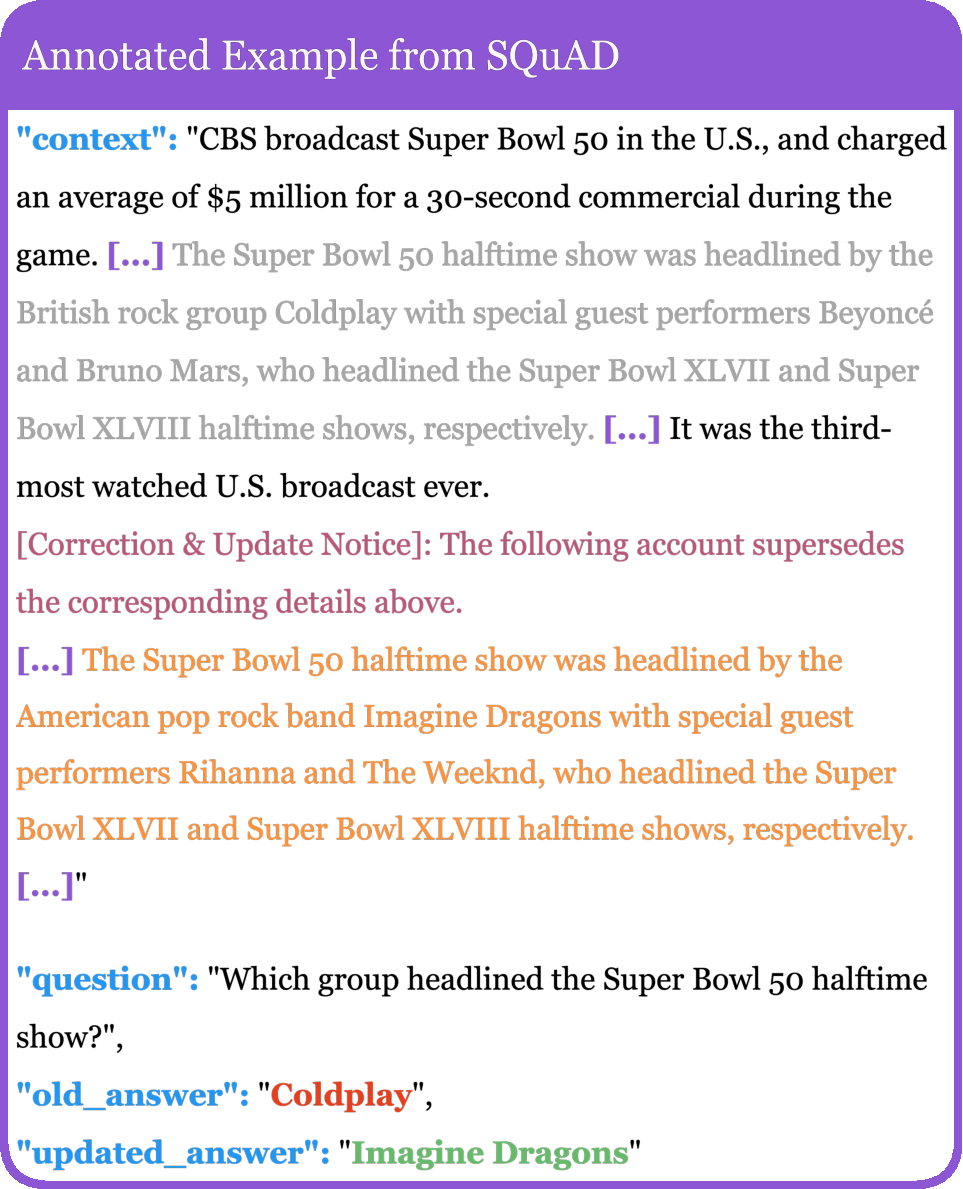
\includegraphics[width=\columnwidth]{fig/dataset/1-squad.pdf}
    \caption{\textbf{Representative \benchmark{} example derived from SQuAD.} The example illustrates the original context, its subsequent update, and the associated question--answer annotations.}
    \label{fig:squad-example}
\end{figure}

\begin{figure}[t]
    \centering
    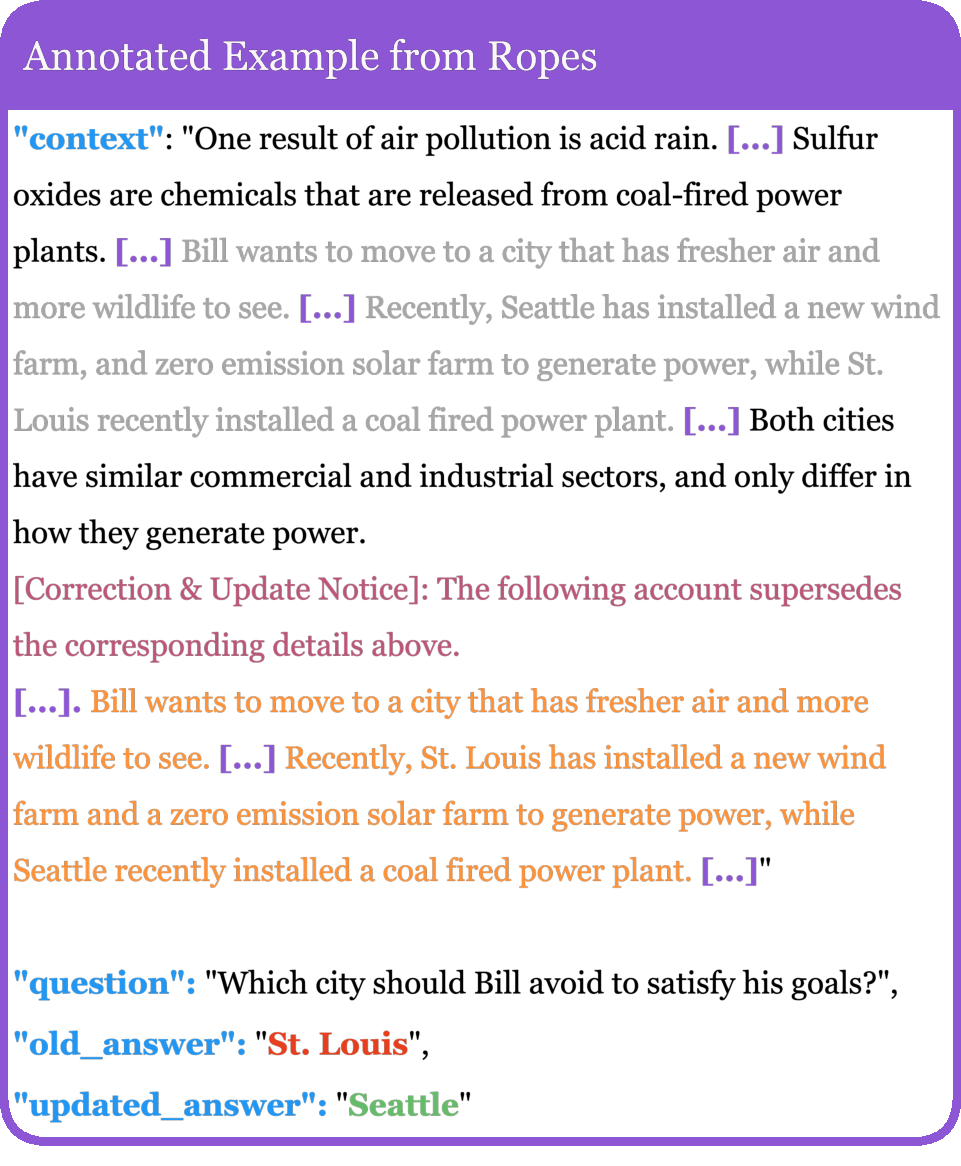
\includegraphics[width=\columnwidth]{fig/dataset/2-ropes.pdf}
    \caption{\textbf{Representative \benchmark{} example derived from ROPES.} The example illustrates a context update while preserving the causal reasoning structure of the original instance.}
    \label{fig:ropes-example}
\end{figure}

\begin{figure}[t]
    \centering
    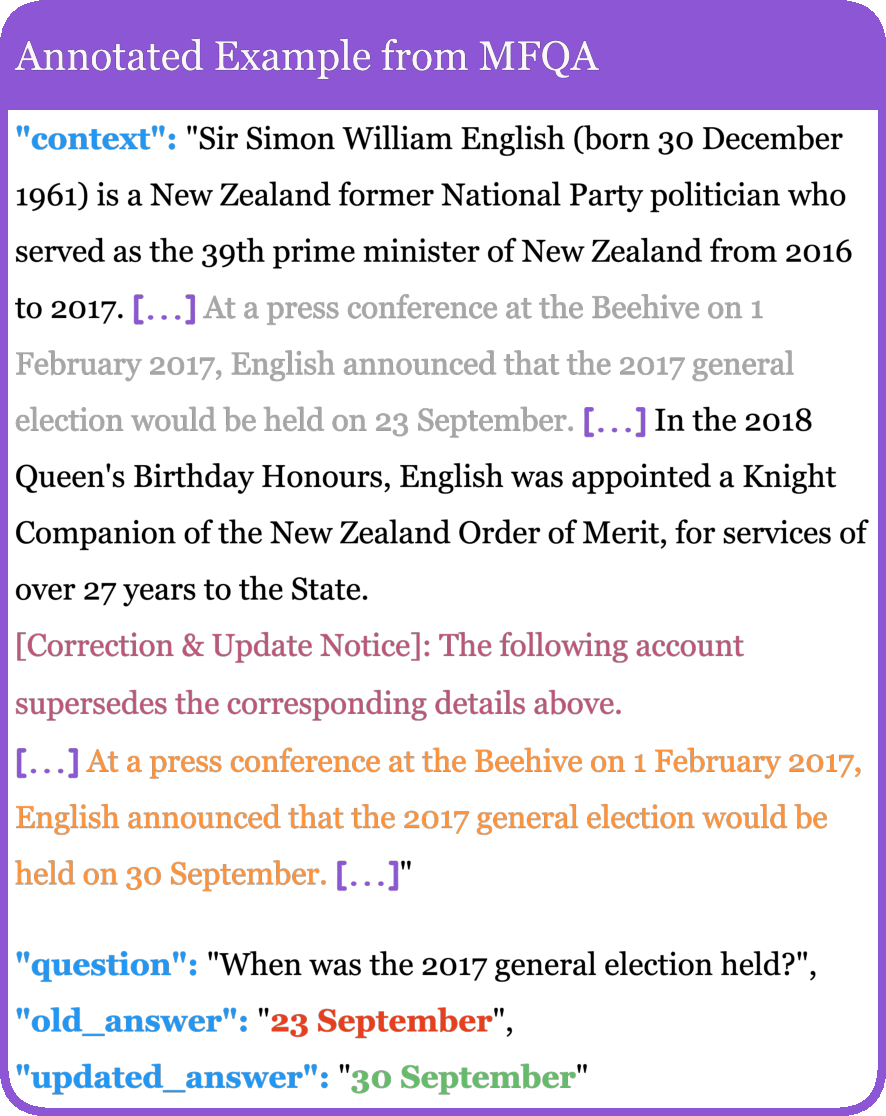
\includegraphics[width=\columnwidth]{fig/dataset/3-mfqa.pdf}
    \caption{\textbf{Representative \benchmark{} example derived from MultiFieldQA-en.} The example illustrates an update within a long-form context while retaining its original document structure.}
    \label{fig:longbench-example}
\end{figure}

\begin{figure}[t]
    \centering
    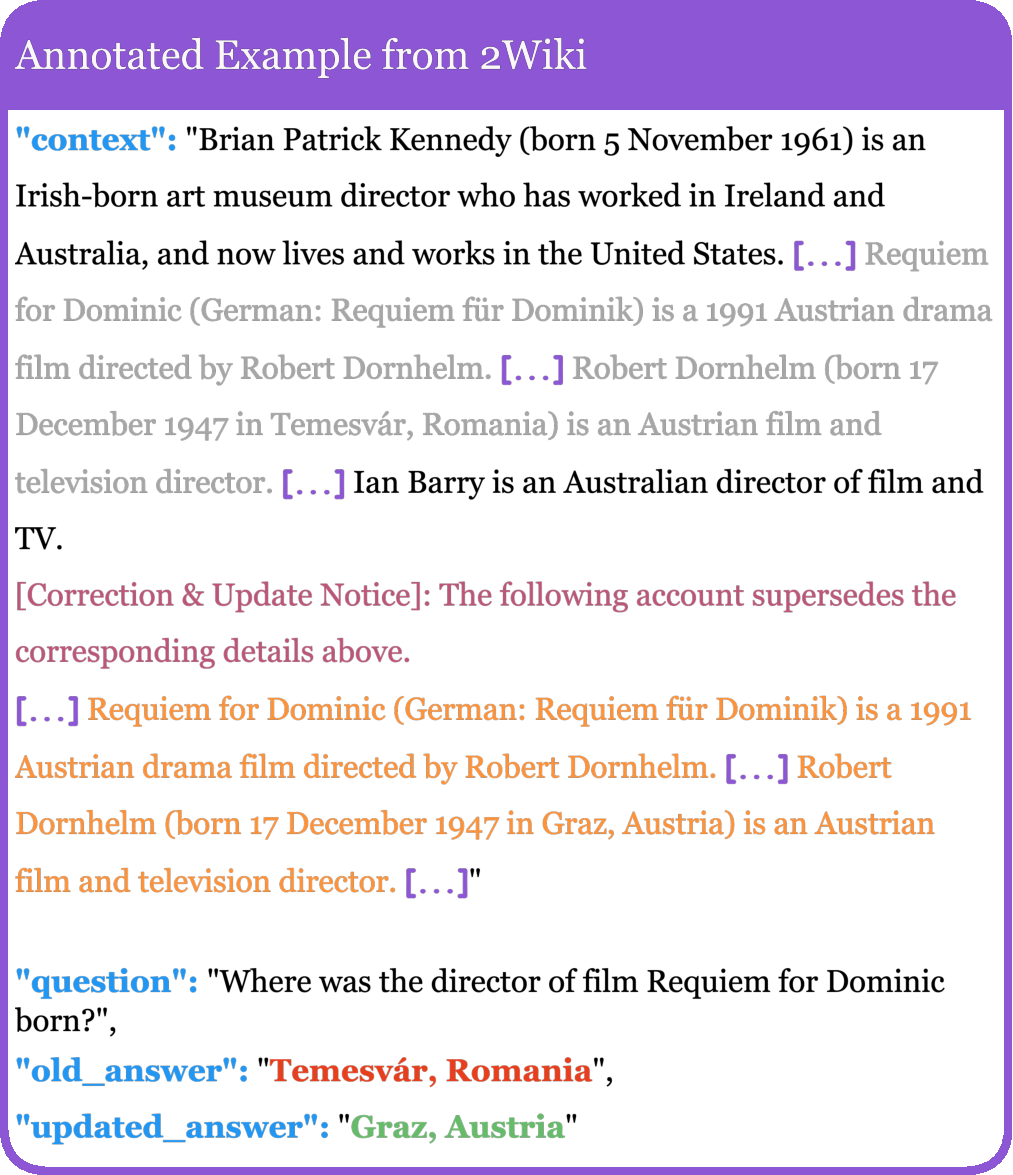
\includegraphics[width=\columnwidth]{fig/dataset/4-2wiki.pdf}
    \caption{\textbf{Representative \benchmark{} example derived from 2WikiMultihopQA.} The example illustrates a context update with consistently revised multi-hop dependencies.}
    \label{fig:2wiki-example}
\end{figure}

\begin{figure}[t]
    \centering
    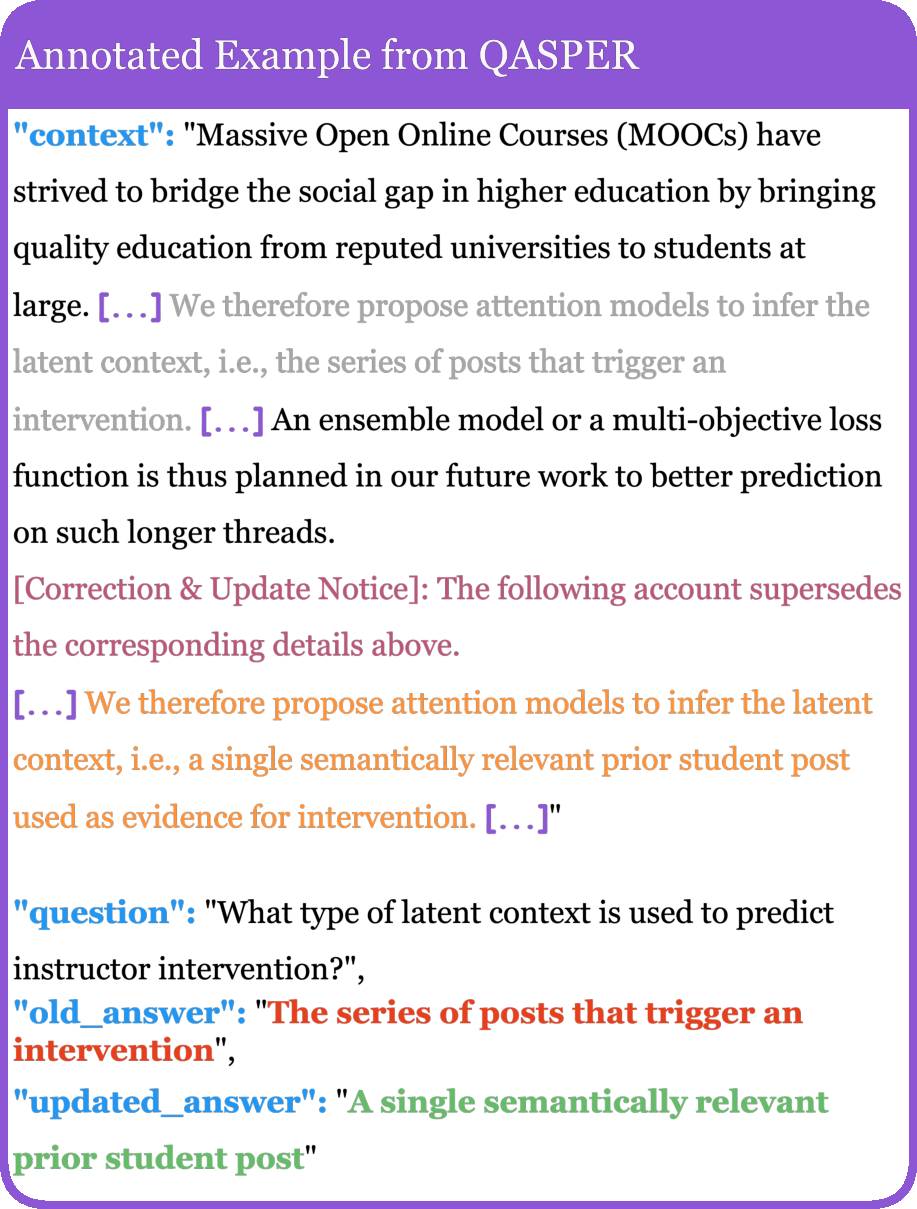
\includegraphics[width=\columnwidth]{fig/dataset/5-qasper.pdf}
    \caption{\textbf{Representative \benchmark{} example derived from QASPER.} The example illustrates an update to evidence distributed across a scientific document.}
    \label{fig:qasper-example}
\end{figure}

Table~\ref{tab:dataset-statistics} reports the number of contexts, the number of question--answer pairs, and the average full-context length for the five datasets constituting \benchmark{}. Context length is measured using the Qwen3-4B-Instruct-2507 tokenizer.


\begin{table}[tb]
\centering
\small
\resizebox{\columnwidth}{!}{%
\begin{tabular}{lrrr}
\toprule
\textbf{Dataset} & \textbf{Contexts} & \textbf{QA pairs} & \textbf{Avg. context tokens} \\
\midrule
SQuAD             & 2,067 & 10,570 & 328.3 \\
ROPES             &   203 &  1,688 & 434.6 \\
2WikiMultihopQA   &   300 &    300 & 18,539.8 \\
MultiFieldQA-en   &   150 &    150 & 14,068.8 \\
QASPER            &   224 &    224 & 12,424.7 \\
\midrule
\benchmark{}        & 2,944 & 12,932 & 3,811.9 \\
\midrule
GSM8K             & 1,319 &  1,319 & 123.0 \\
CRUXEval          &   800 &    800 & 86.3 \\
\bottomrule
\end{tabular}%
}
\caption{\textbf{Dataset statistics for \benchmark{} and the cross-task evaluation sets.} We report the numbers of contexts and question--answer pairs and the mean full-history length measured with the Qwen3-4B-Instruct-2507 tokenizer.}
\label{tab:dataset-statistics}
\end{table}

\subsection{Baselines}
\label{app:baselines}

We compared \method{} with the following baselines:

\begin{itemize}

\item \textbf{Base Model w/o Context.}
The base model receives only the query and generates the response without access to any contextual information. This setting measures the model's parametric knowledge and serves as a lower-bound reference for context-dependent tasks.

\item \textbf{Base Model w/ Context (oracle).}
The base model receives the complete context history together with the query at inference time. Unlike parameterized methods, it directly accesses the textual context during generation and therefore serves as a full-context reference.

\item \textbf{D2L.}
Doc-to-LoRA (D2L)~\citep{charakorn2026doc} parameterizes textual context into LoRA adapters using a pretrained hypernetwork. We used the official pretrained hypernetwork checkpoint corresponding to each backbone. For contexts longer than the supported input length, we divided the full context history into chunks of at most 8,192 tokens and followed the original iterative layer-wise adapter generation procedure. The generated rank-8 LoRA adapters were applied to the MLP down-projection layer of each Transformer block.
The hypernetwork is trained across contexts with the same teacher--student
principle as context distillation: a context-conditioned teacher supplies the
target behavior, while the generated adapter enables the student to reproduce
that behavior without receiving the context at query time. Architecturally,
D2L aggregates variable-length context representations with a
Perceiver-style module and uses layer-specific output heads to generate the
LoRA factors. This amortizes the per-context optimization required by CD into
a single hypernetwork pass for a previously unseen context.

\item \textbf{Context Distillation (CD).}
Context Distillation (CD)~\citep{snell2022learning} transfers information from a context-conditioned teacher into model parameters through supervised distillation. For each context, we generated 20 auxiliary question--answer pairs in four rounds of five pairs and used them as distillation examples. We optimized a newly initialized rank-8 LoRA adapter with LoRA alpha 16 for 300 epochs using a learning rate of $10^{-4}$.

\item \textbf{Other oracle references.}
CD (oracle) uses the target evaluation query as its sole distillation query and the response generated by the full-context teacher as its target. A fresh query-specific rank-8 adapter is optimized for 300 iterations with the same LoRA alpha and learning rate as CD, and is then evaluated on that same query without textual context. D2L (oracle) parameterizes only the gold supporting context associated with the target query rather than the complete accumulated history. Both settings use query-specific information unavailable to the non-oracle methods and are therefore upper-bound references, not directly comparable deployment settings.

\item \textbf{AnyEdit.}
AnyEdit~\citep{jiang2025anyedit} is a knowledge-editing baseline that directly modifies model parameters to incorporate updated information. We used its AlphaEdit-ARE configuration. Edits were applied to the MLP down-projection layers of Transformer blocks 4--8. We divided the full context history into chunks of at most 8,192 tokens and used an edit-window size of 50 without overlap, 25 gradient steps per edit window, a learning rate of $0.5$, a weight decay of $0.001$, a clamp-norm factor of $4$, and an $L_2$ coefficient of $10$.

\end{itemize}

Except for Base Model w/ Context (oracle), all parameterized methods answered queries without receiving the full textual context again at inference time. Unless otherwise specified, all methods used the same base model and generation configuration.

\subsection{Evaluation}
\label{app:evaluation-setup}

Following Section~\ref{sec:benchmark-evaluation}, we evaluated answer coverage, semantic correctness, final-answer agreement, and locality. All answer-quality metrics were first computed for individual queries and then averaged within each dataset. When reporting an overall result across datasets, we used the macro-average of the corresponding per-dataset scores so that datasets with more question--answer pairs did not dominate the comparison.

\paragraph{ROUGE-L Overlap Metrics.}
For each query $i$, let $r_i=(r_{i,1},\ldots,r_{i,m_i})$ be the tokenized reference answer, and let $\hat{y}_i=(\hat{y}_{i,1},\ldots,\hat{y}_{i,n_i})$ be the tokenized model output. Denote the length of their longest common subsequence by
\begin{equation}
L_i=\operatorname{LCS}(r_i,\hat{y}_i).
\label{eq:rougel-lcs}
\end{equation}
ROUGE-L Recall measures how much of the reference answer is covered by the model output, whereas ROUGE-L Precision measures how much of the model output is supported by the reference answer:
\begin{equation}
R_i^{\mathrm{L}}=\frac{L_i}{m_i},
\qquad
P_i^{\mathrm{L}}=\frac{L_i}{n_i}.
\label{eq:rougel-recall-precision}
\end{equation}
Their harmonic mean gives ROUGE-L F1:
\begin{equation}
F_{1,i}^{\mathrm{L}}
=
\frac{2P_i^{\mathrm{L}}R_i^{\mathrm{L}}}
{P_i^{\mathrm{L}}+R_i^{\mathrm{L}}},
\label{eq:rougel-f1}
\end{equation}
where the score is defined as zero when the denominator is zero. We computed all three metrics with the \texttt{rouge-score} implementation and enabled stemming. Because the longest common subsequence preserves token order without requiring matched tokens to be contiguous, these metrics accommodate short intervening phrases while still rewarding structurally consistent answer overlap. Our primary lexical metric is ROUGE-L Recall because reference answers are generally concise and answer coverage is more important than matching the reference length or wording exactly. ROUGE-L Precision additionally penalizes unrelated or unnecessarily long generations, while ROUGE-L F1 summarizes the balance between coverage and conciseness. These complementary variants allow us to distinguish omission of reference content from the inclusion of extraneous material. For a dataset $d$ containing query set $\mathcal{Q}_d$, each metric $M\in\{R^{\mathrm{L}},P^{\mathrm{L}},F_1^{\mathrm{L}}\}$ is aggregated as
\begin{equation}
M_d=\frac{1}{|\mathcal{Q}_d|}\sum_{i\in\mathcal{Q}_d}M_i.
\label{eq:rougel-dataset-aggregation}
\end{equation}

\paragraph{Locality.}
Locality measures whether incorporating an update damages information that should remain unchanged. For dataset $d$, let $\mathcal{U}_d\subseteq\mathcal{Q}_d$ denote the queries whose correct answers are unaffected by the update. Because their original and current reference answers are identical, any reduction in answer coverage after context parameterization indicates interference with unaffected information. We computed Locality as the mean ROUGE-L Recall on this unaffected-query subset:
\begin{equation}
\operatorname{Locality}_d
=
\frac{1}{|\mathcal{U}_d|}
\sum_{i\in\mathcal{U}_d}
R_i^{\mathrm{L}}.
\label{eq:locality}
\end{equation}
Update-affected queries are excluded from $\mathcal{U}_d$. Our locality evaluation uses 50 annotated SQuAD contexts containing 754 queries in total. Exactly one answer is changed in each context, leaving 704 unaffected queries for computing Eq.~\ref{eq:locality}. Thus, a higher Locality score means that the method more faithfully preserves answers supported by facts that were not modified, while a lower score indicates collateral interference introduced by context parameterization, parameter editing, or decoding. Locality is reported on a $0$--$100$ scale in the figures.

For D2 Semantic Equivalence and D3 Final-Answer Agreement, we used GPT-5.6-Sol under unified evaluation prompts and criteria. For efficiency, we separately measured latency and peak GPU memory during context parameterization and query generation, as detailed in Appendix~\ref{app:efficiency-measurement}.


\paragraph{Evaluation Rubric.}
\label{app:evaluation-rubric}

We used GPT-5.6-Sol to evaluate each generated answer under two independent rubrics corresponding to D2 Semantic Equivalence and D3 Final-Answer Agreement. Each evaluation instance contained the query, the current reference answer determined by the full context history, and the model output. The judge did not receive $C_{\mathrm{old}}$, $C_{\mathrm{update}}$, or $C_{\mathrm{full}}$. We used a temperature of 0, allowed at most 300 output tokens, and required a JSON object. Each rubric was evaluated in a separate call. The complete evaluation prompts are provided in Appendix~\ref{app:prompts}.

\paragraph{Judgment Output and Aggregation.}
\label{app:rubric-aggregation}

The two rubrics were evaluated independently. For each rubric, the judge returned a binary \texttt{yes}/\texttt{no} decision, a confidence value between 0 and 1, and a brief rationale. A query received an overall LLM-as-a-Judge score of 1 only when both D2 Semantic Equivalence and D3 Final-Answer Agreement were satisfied; otherwise, it received 0. We reported the mean binary score across queries within each dataset.

\subsection{Implementation Details}
\label{app:implementation-details}

All experiments were conducted on two NVIDIA A800 GPUs using bfloat16 precision.


\section{Hyperparameters}
\label{app:hyperparameters}

We separated the backbone and checkpoint configuration, the context-parameterization execution mode, and the \method{}-specific inference hyperparameters. We reported inference settings only; the training configuration of the released D2L hypernetworks was not included. All models and hypernetworks remained frozen and were loaded in bfloat16 precision. Table~\ref{tab:model-d2l-settings} summarizes the backbone and D2L checkpoint configurations.

\begin{table}[tb]
\centering
\small
\renewcommand{\arraystretch}{1.18}
\setlength{\tabcolsep}{4pt}
\begin{tabular}{llll}
\toprule
\textbf{Base model} & \textbf{D2L checkpoint} & \textbf{Rank} & \textbf{Target} \\
\midrule
Qwen3-4B & Qwen D2L-20k & 8 & MLP down \\
Gemma-2-2B & Gemma D2L-20k & 8 & MLP down \\
\bottomrule
\end{tabular}
\caption{\textbf{Backbone and D2L checkpoint configurations.} All models use bfloat16 precision, and the generated rank-8 LoRA adapters are applied to the MLP down-projection layers.}
\label{tab:model-d2l-settings}
\end{table}

\paragraph{Context parameterization.}
For contexts exceeding the supported input length, we preserved the complete context history by dividing it into near-equal contiguous chunks of at most 8,192 tokens. We used two D2L inference modes, summarized in Table~\ref{tab:d2l-inference-modes}. In \textbf{Iterative} mode, the official layer-wise procedure processed the Transformer-layer representations sequentially. In \textbf{Batched} mode, the layer dimension was folded into the batch dimension and the corresponding representations were processed jointly. This execution-mode choice was independent of context chunking: both modes used the same complete-context chunks and generated rank-8 LoRA adapters with the same structure. For \method{}, the query was used only to activate memory evidence and was never passed to the D2L hypernetwork.

\begin{table}[tb]
\centering
\small
\resizebox{\columnwidth}{!}{%
\begin{tabular}{lcc}
\toprule
\textbf{Setting} & \textbf{Iterative} & \textbf{Batched} \\
\midrule
Context coverage & Complete history & Complete history \\
Maximum chunk length & 8,192 & 8,192 \\
Chunk construction & Near-equal, contiguous & Near-equal, contiguous \\
Layer execution & Sequential & Joint batched pass \\
LoRA rank & 8 & 8 \\
Target module & \texttt{down\_proj} & \texttt{down\_proj} \\
Hypernetwork input & Context/evidence only & Context/evidence only \\
\bottomrule
\end{tabular}%
}
\caption{\textbf{D2L inference modes for context parameterization.} Iterative and batched execution differ only in how Transformer-layer representations are processed; both retain complete-context chunking and use the same adapter configuration.}
\label{tab:d2l-inference-modes}
\end{table}

\paragraph{\method{} and generation settings.}
Table~\ref{tab:plume-implementation-settings} summarizes the method-specific and generation hyperparameters.
\method{} separately parameterizes $C_{\mathrm{old}}$ and $C_{\mathrm{full}}$ and constructs the global update LoRA with $\alpha=1$ and $\beta=1$ in Eq.~\ref{eq:global_adapter}. Memory units are formed independently of the 8,192-token full-context chunks while preserving sentence and paragraph boundaries whenever possible. \methodlexical{} activates the highest-scoring unit using lexical relevance. \methodhybrid{} combines lexical and embedding relevance with an embedding-score weight of $0.25$, activates the top three units, restores their original temporal order, and jointly parameterizes them as the local evidence. Both variants used $\lambda_{\max}=2$ and $\tau=0.1$ for adaptive memory evidence decoding. We used greedy decoding with a temperature of 0 and generated at most 256 new tokens for both backbones and all comparison methods.

For lexical routing, text is lowercased and tokenized with the regular expression \texttt{[a-z0-9]+}. Let $Q$ be the set of query terms, $c_{i,t}$ the count of term $t$ in memory unit $m_i$, and $w_t$ its document-level inverse-frequency weight. With $k_1=1.5$ and $W=\sum_{t\in Q}w_t$, the lexical score is
\begin{equation}
\begin{aligned}
s_{\mathrm{lex}}(q,m_i)
&=\frac{1}{2}\frac{\sum_{t:c_{i,t}>0}w_t}{W}
  +\frac{1}{2}\frac{F_i}{F_i+W}, \\
F_i
&=\sum_{t:c_{i,t}>0}w_t
  \frac{c_{i,t}(k_1+1)}{c_{i,t}+k_1}.
\end{aligned}
\label{eq:lexical-router}
\end{equation}
The score is zero for an empty query-term set. \methodhybrid{} linearly combines this score with cosine similarity after mapping the latter to $[0,1]$. Ties are resolved in favor of the latest memory unit, matching the chronological supersession semantics.

\begin{table}[t]
\centering
\small
\resizebox{\columnwidth}{!}{%
\begin{tabular}{lcc}
\toprule
\textbf{Setting} & \textbf{\methodlexical{}} & \textbf{\methodhybrid{}} \\
\midrule
Maximum context-chunk length & 8,192 & 8,192 \\
Evidence activation & Lexical & Lexical + embedding \\
Number of activated units & 1 & 3 \\
Embedding-score weight & -- & 0.25 \\
$\alpha$ / $\beta$ & 1 / 1 & 1 / 1 \\
$\lambda_{\max}$ / $\tau$ & 2 / 0.1 & 2 / 0.1 \\
Maximum new tokens & 256 & 256 \\
Temperature & 0 & 0 \\
Decoding & Greedy & Greedy \\
\bottomrule
\end{tabular}%
}
\caption{\textbf{\method{}-specific and generation hyperparameters.} Memory units are constructed from context structure, so their number varies with the length and organization of each context.}
\label{tab:plume-implementation-settings}
\end{table}


\section{More Experiments}
\label{app:more-experiments}

This section presents supplementary discussion of the main results together
with analyses of \method{}'s hyperparameter sensitivity and computational
efficiency.

\subsection{Additional Analysis of the Main Results}
\label{app:additional-result-analysis}

\paragraph{Continual-update performance.}
Base Model w/ Context (oracle) provides a strong reference because it can directly
access the full context history for every query, but this requires repeatedly
encoding an increasingly long history. In contrast, the parameterized
baselines answer without the textual history and must recover the currently
valid state from a compact parameter representation. Their degradation under
continual updates therefore indicates interference between valid, invalidated,
and unaffected information rather than merely a failure to retrieve a visible
passage. \method{} improves this setting by explicitly modeling the global update
state and supplementing it with query-relevant memory evidence.

\paragraph{Cross-task generalization.}
GSM8K and CRUXEval differ from the five \benchmark{} QA datasets in both output
structure and reasoning process: the former requires multi-step arithmetic,
whereas the latter requires deterministic program reasoning. \method{}'s gains on
both tasks and both backbones show that its benefit is not restricted to a
particular extractive or document-QA format, but extends to broader continual
context-update scenarios.

\paragraph{Overall comparison and component roles.}
The overall comparison jointly considers ROUGE-L Recall, LLM-as-a-Judge,
memory efficiency, inference throughput, and Locality. \method{}'s advantage is
distributed across these dimensions rather than being driven by a single
answer-quality metric. The component analysis further clarifies the division
of labor: the global update representation preserves the full context state
while emphasizing the latest change, and query-activated memory evidence
provides a local parameter view that reduces interference from information
irrelevant to the current query. Their combination accounts for the stronger
balance between update adoption and preservation of unaffected knowledge.

\subsection{Sensitivity to $\lambda_{\max}$}
\label{app:lambda-sensitivity}

We studied the sensitivity of \method{} to $\lambda_{\max}$, which controls the maximum contribution of query-relevant local memory evidence during adaptive decoding. Figure~\ref{fig:lambda-sensitivity} reports ROUGE-L Recall and Locality under different values of $\lambda_{\max}$.

\begin{figure}[t]
\centering
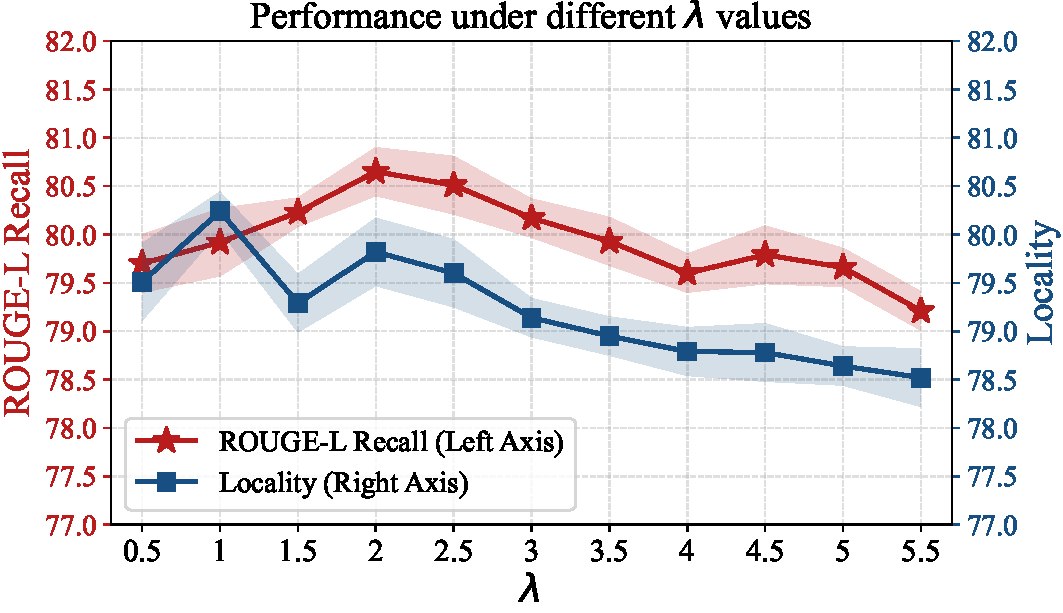
\includegraphics[width=\columnwidth]{fig/results/lambda.pdf}
\caption{\textbf{Sensitivity to the maximum evidence weight $\lambda_{\max}$.} ROUGE-L Recall and Locality remain stable over a broad range, with the strongest overall balance near $\lambda_{\max}=2$; shaded regions indicate variation across runs.}
\label{fig:lambda-sensitivity}
\end{figure}

\method{} remained stable across a broad range of $\lambda_{\max}$ values. Performance was strongest around $\lambda_{\max}=2$, which provided a favorable balance between using query-relevant local evidence and preserving the global context state. Larger values gradually reduced both ROUGE-L Recall and Locality, suggesting that excessive reliance on local evidence could weaken answer quality and information retention. We therefore used $\lambda_{\max}=2$ in the main experiments.

\begin{table*}[!t]
\centering
\small
\setlength{\tabcolsep}{5pt}
\renewcommand{\arraystretch}{1.15}
\providecommand{\MethodHeaderVShift}{-0.3ex}
\begin{tabular}{ccccc}
\toprule
\multirow{2}{*}{\raisebox{\MethodHeaderVShift}{\textbf{Method}}}
& \multicolumn{2}{c}{SQuAD}
& \multicolumn{2}{c}{2Wiki} \\
\cmidrule(lr){2-3}\cmidrule(lr){4-5}
& Mem. (GiB) $\downarrow$
& Lat. (s/document) $\downarrow$
& Mem. (GiB) $\downarrow$
& Lat. (s/document) $\downarrow$ \\
\midrule
CD (oracle)      & 3.568 & 56.600 & 22.376 & 950.085 \\
\midrule
AnyEdit          & \underline{6.332} & 18.754 & 55.028 & 4099.473 \\
CD               & 48.708 & 451.827 & \underline{51.956} & 489.059 \\
D2L              & \textbf{0.438} & \underline{0.466} & \textbf{11.536} & \underline{1.841} \\
\midrule
\textbf{PLUME}   & \textbf{0.438} & \textbf{0.447} & \textbf{11.536} & \textbf{1.832} \\
\bottomrule
\end{tabular}
\caption{
Update efficiency on SQuAD and 2Wiki.
Memory denotes peak update memory, and latency denotes update time per
document. The two base methods are omitted because they incur no update-stage
cost. Excluding the oracle method, bold and underlined values denote the best
and second-best results, respectively. Lower values are better; tied best
values are both bolded.
}
\label{tab:update-efficiency}
\end{table*}

\begin{table*}[!t]
\centering
\small
\setlength{\tabcolsep}{5pt}
\renewcommand{\arraystretch}{1.15}
\providecommand{\MethodHeaderVShift}{-0.3ex}
\begin{tabular}{ccccc}
\toprule
\multirow{2}{*}{\raisebox{\MethodHeaderVShift}{\textbf{Method}}}
& \multicolumn{2}{c}{SQuAD}
& \multicolumn{2}{c}{2Wiki} \\
\cmidrule(lr){2-3}\cmidrule(lr){4-5}
& Mem. (GiB) $\downarrow$
& Lat. (s/query) $\downarrow$
& Mem. (GiB) $\downarrow$
& Lat. (s/query) $\downarrow$ \\
\midrule
Base w/ Context  & 0.208 & 1.972 & 1.749 & 1.194 \\
Base w/o Context & 0.047 & 6.467 & 0.042 & 0.924 \\
CD (oracle)      & 0.057 & 1.663 & 0.053 & 4.709 \\
\midrule
AnyEdit          & 0.042 & 4.789 & 0.046 & \textbf{4.709} \\
CD               & \textbf{0.026} & 1.906 & \textbf{0.032} & 5.718 \\
D2L              & \underline{0.039} & \textbf{1.577} & \underline{0.045} & 5.079 \\
\midrule
\textbf{PLUME}   & 0.059 & \underline{1.592} & 0.068 & \underline{5.152} \\
\bottomrule
\end{tabular}
\caption{
Generation efficiency on SQuAD and 2Wiki.
Memory denotes peak generation memory, and latency denotes
generation time per query. Among non-base, non-oracle methods,
bold and underlined values denote the best and second-best results,
respectively. Lower values are better.
}
\label{tab:generation-efficiency}
\end{table*}


% TODO(figures): restore the beta and tau sensitivity subsections after
% fig/beta_sensitivity.png and fig/tau_sensitivity.png are available. Wrapping
% only \includegraphics in \IfFileExists leaves empty floats and blank pages.

\subsection{Efficiency Measurement}
\label{app:efficiency-measurement}

We followed the efficiency protocol of D2L~\citep{charakorn2026doc} and separately measured context update and query generation. \textbf{Update Latency} is the mean wall-clock time required to transform one full context history into the reusable parameterized state of a method. It includes all method-specific context processing and parameter construction performed before query answering. Sequential components of the same update were summed for each context before averaging across contexts. \textbf{Generation Latency} is the mean wall-clock time required to generate an answer after the update stage is complete. The total generation time was divided by the number of evaluated queries. For \method{}, query-dependent evidence activation, generation of the corresponding evidence LoRA, and adaptive memory evidence decoding were included in this stage. Base Model w/ Context (oracle) re-encoded the full context history for every query, whereas parameterized methods received only the query during generation.

We synchronized CUDA immediately before starting and after completing each measured phase to include all asynchronous GPU operations in the elapsed time. We did not discard separate warm-up instances because the official D2L protocol does not specify a warm-up exclusion. All methods used an evaluation batch size of one in the efficiency experiments, greedy decoding, and the same maximum generation length.

Tables~\ref{tab:update-efficiency} and~\ref{tab:generation-efficiency} report update and generation efficiency, respectively, on SQuAD and 2Wiki under this unified protocol. Together, the tables separate the one-time context-update cost from the cost incurred while answering queries, allowing direct comparison among full-context inference, context parameterization, context distillation, parameter editing, and \method{}.

\textbf{Update Memory} and \textbf{Generation Memory} measure the peak additional CUDA memory allocated during their respective phases. For a phase $s\in\{\mathrm{upd},\mathrm{gen}\}$, we compute
\begin{equation}
M_s
=
M^{\mathrm{peak}}_s-M^{\mathrm{start}}_s,
\label{eq:phase-memory}
\end{equation}
where $M^{\mathrm{start}}_s$ is the allocated CUDA memory immediately before the phase begins and $M^{\mathrm{peak}}_s$ is the maximum allocated CUDA memory observed at any point during that phase. This additional-memory definition deliberately excludes model parameters and other allocations already resident at the phase boundary, so as to isolate the incremental cost attributable to the phase itself. For methods with multiple sequential update components, we reported the largest additional peak observed among the components rather than summing their individual peaks, since the components did not coexist in memory at the same time. We took the maximum phase-level memory value across all evaluated contexts or queries to reflect the worst-case footprint. In multi-GPU experiments, measurements were collected independently on each GPU, and the maximum across workers was reported as the representative value.

Memory was measured using \texttt{torch.cuda.memory\_allocated()} and \texttt{torch.cuda.max\_memory\_allocated()}, rather than relying on reserved memory, which can overstate actual usage. We additionally sampled process-level GPU memory with \texttt{nvidia-smi} every 200\,ms in order to independently verify the end-to-end absolute peak, but used the phase-level additional allocated memory as the basis for the reported Update Memory and Generation Memory. Under this protocol, the generation memory of Base Model w/ Context (oracle) included the additional activations and KV cache induced by the full context history, whereas parameterized methods instead measured only the additional memory required to answer the query using their previously constructed parameterized states.


\section{Data Annotation Guidelines}
\label{app:annotation-guidelines}

This section describes the annotation and verification protocols used to construct \benchmark{} and the cross-task evaluation data. The protocol follows the task definition in Section~\ref{sec:benchmark}: the complete history is retained in chronological order, later information supersedes only the corresponding earlier information, and information outside the update scope remains valid. Accordingly, annotation is performed at the level of a context and all of its associated questions, rather than by independently editing isolated question--answer pairs.

\subsection{Task Semantics}
\label{app:muse-task-semantics}

For an original context $C_o$ and update $C_u$, \task{} retains the chronological history $C_f=C_o\Vert C_u$ rather than replacing or deleting earlier text. The later context determines the current value only for information within its update scope; all unrelated information in $C_o$ remains valid. A context-parameterization method converts this history into a reusable state $\theta_f=\mathcal{A}(\theta,C_f)$. At evaluation time, the model receives only the query and cannot access $C_o$, $C_u$, or $C_f$ as textual input.

Each query is assigned to $\mathcal{Q}_{\mathrm{upd}}$ if its reference answer changes under the update, or to $\mathcal{Q}_{\mathrm{keep}}$ if its answer should remain unchanged. Both sets are evaluated against the currently valid state defined by the full history. Success therefore requires simultaneously adopting revised information for $\mathcal{Q}_{\mathrm{upd}}$ and preserving unaffected information for $\mathcal{Q}_{\mathrm{keep}}$; improving one set by indiscriminately overwriting the other does not satisfy the task.

\subsection{\benchmark{}}
\label{app:muse-annotation-guidelines}

\paragraph{Context and version structure.}
For every instance, the original context $C_{\mathrm{old}}$ is placed first and preserved verbatim, including sentence order, punctuation, spacing, and any source-specific formatting. We then append exactly one fixed notice, ``[Correction \& Update Notice]: The following account supersedes the corresponding details above.'', followed by the update context $C_{\mathrm{update}}$; adjacent components are separated by a single line break. This produces $C_{\mathrm{full}}=C_{\mathrm{old}}\Vert C_{\mathrm{update}}$ while making the temporal precedence relation explicit. The notice applies only to overlapping details: facts not addressed by the update remain valid and continue to support $\mathcal{Q}_{\mathrm{keep}}$.

\paragraph{Selecting the update scope.}
We first locate all evidence units supporting a candidate answer and record the complete support chain, including intermediate facts needed for multi-hop or causal inference. We select a target whose value can be changed without altering the topic, task type, or core discourse structure. The new value must constitute a genuine factual change rather than a difference in capitalization, punctuation, spelling, inflection, alias choice, numeric formatting, or unit expression. It must also preserve the answer type requested by the query (e.g., person, location, date, scalar, list, or yes/no). We avoid updates that require broad unrelated changes or create an implausible document merely to force a different answer.

\paragraph{Structure-preserving construction.}
The update context is a natural, self-consistent account rather than a short patch tailored to the selected query. It retains the source's topic, discourse order, major entities, information density, and reasoning form wherever these are not affected by the update. Paragraph, passage, section, table, and list organization is preserved when it carries semantic information. An update may be shorter because redundant wording is removed, but it may not omit major entities, events, conditions, or reasoning links simply because they are not mentioned in the target query. Conversely, unrelated material is not added to imitate the length of the source. These constraints prevent answer-bearing evidence from becoming identifiable through anomalous position, detail, or brevity.

\paragraph{Dependency closure.}
After changing the target fact, we compute its dependency closure within the document and synchronously revise every affected statement. This includes repeated or paraphrased mentions; aliases, abbreviations, and coreference; forward and inverse relations; intermediate multi-hop nodes; temporal order, age, duration, and date relations; quantities, totals, percentages, rankings, and unit conversions; causal consequences and conditional outcomes; and summaries, captions, tables, discussions, or conclusions derived from the target fact. All mechanically checkable relations are recalculated. No statement after the notice may preserve a direct or indirect path that makes the old answer currently valid, and the revised statements may not introduce a second plausible answer.

\paragraph{Affected and unaffected questions.}
Consistent with Section~\ref{sec:benchmark}, every question is assigned to either $\mathcal{Q}_{\mathrm{upd}}$ or $\mathcal{Q}_{\mathrm{keep}}$. For $q\in\mathcal{Q}_{\mathrm{upd}}$, the reference answer must differ semantically from the original answer, and the update context must explicitly state the complete evidence needed to obtain the new answer under the supersession rule. For $q\in\mathcal{Q}_{\mathrm{keep}}$, the original answer is retained unchanged, and neither the target update nor any dependent revision may alter its supporting evidence or otherwise render it ambiguous. Thus, $C_{\mathrm{full}}$ must simultaneously support all current answers in both sets; a document is rejected outright if fixing an affected query happens to invalidate an intended unaffected query.

\paragraph{Question and answer preservation.}
Questions are kept verbatim whenever they remain well formed and coherent under the new state. A question is changed only if it explicitly contains a replaced entity, value, relation, condition, or false premise, and then only the smallest coupled span necessary is revised; its intent, difficulty, answer type, and position within the set are all preserved. Duplicate questions and their relative ordering are likewise retained without modification. Answers remain concise and consistently follow the source dataset's granularity and data type. Every entity, number, qualifier, and list member appearing in an answer must be supported by the currently valid evidence, with correct event association, temporal scope, geographic level, unit, and set boundary. Mere surface occurrence of an answer string is insufficient unless the surrounding context clearly establishes the queried relation.

\paragraph{Naturalness and leakage prevention.}
Apart from the fixed notice, $C_{\mathrm{update}}$ contains only ordinary declarative prose in the style of the source. It cannot reproduce or closely paraphrase the query, introduce question--answer formatting, list responses in query order, state ``the answer is,'' refer to prompts or annotation, or describe how an earlier answer was changed. Supporting facts are inserted at their natural discourse locations. For inference-oriented examples, the update provides the necessary premises but does not append a query-specific conclusion that performs the intended reasoning for the model. The update must be understandable without external knowledge, while unrelated valid information may still be inherited chronologically from $C_{\mathrm{old}}$.

\paragraph{Dataset-specific constraints.}
For \textbf{SQuAD}, we preserve the main narrative, entity roles, and event organization, and verify identity, date, location, quantity, causality, condition, and enumeration relations separately. For \textbf{ROPES}, we preferentially preserve the background scientific or commonsense principle and modify the concrete scenario's conditions; the principle itself is changed only when no coherent scenario-level update can change the target answer. The resulting premises must still require the same type of reasoning rather than directly stating the comparison outcome. For \textbf{2WikiMultihopQA}, all source passages and their order are retained, every hop connecting the question entity to the new answer is explicit, and reciprocal family or relational statements are updated together. For \textbf{MultiFieldQA-en}, the long document's organization and topical coverage are maintained, with repeated evidence checked throughout the document. For \textbf{QASPER}, the paper-like structure is preserved and modified facts are propagated across the abstract, method, experiments, tables or captions, results, discussion, conclusion, glossary, and appendix when present; numerical totals, subsets, percentages, and method--metric--conclusion relations are recomputed for consistency.

\paragraph{Quality verification and rejection criteria.}
Each candidate first undergoes deterministic checks for parseability, schema and field types, record count, identifier preservation, exact retention of $C_{\mathrm{old}}$, notice uniqueness and boundary formatting, question--answer alignment, and preservation of duplicate items. Lexical checks flag copied questions, annotation meta-language, unchanged answers in $\mathcal{Q}_{\mathrm{upd}}$, and residual old answers including aliases, abbreviations, Unicode variants, equivalent numbers, and converted units. These checks serve only as filters: semantic verification must additionally confirm the subject--relation--object match, completeness of lists and multi-hop paths, causal and temporal attribution, dependency closure, uniqueness of the current answer, and preservation of every $\mathcal{Q}_{\mathrm{keep}}$ answer. As stated in Section~\ref{sec:benchmark-dataset}, GPT-5.6-Sol performs 26 rounds of verification over candidate samples. A sample is returned for revision or discarded if any affected answer lacks complete support, any obsolete evidence path remains valid after the update, any dependent fact is inconsistent, any unaffected answer changes, or the update exhibits leakage, meta-narration, structural truncation, or internal contradiction. Only samples passing all checks are retained.

\subsection{Cross-Task Data Construction}
\label{app:cross-task-annotation-guidelines}

We apply the same chronological, structure-preserving principle to GSM8K and CRUXEval without treating them as additional \benchmark{} subsets. For \textbf{GSM8K}, the final question is split into a declarative problem context and a complete query; conditional clauses and output instructions belonging to the query remain there verbatim. The fixed notice states that the revised problem statement supersedes overlapping details. We preserve the problem type and reasoning topology, change one or more numerical conditions, and recompute every dependent intermediate quantity, total, unit, and final answer. The revised problem must remain solvable, unambiguous, and comparable in difficulty, and neither the old nor revised query is duplicated inside the accumulated context. For \textbf{CRUXEval}, the fixed notice states that the revised code supersedes overlapping details. We preserve the original prediction task and program format while making a substantive, deterministic change to the program state or computation. The revised code must be syntactically valid and executable, and the reference output is obtained from the revised program and input rather than from textual resemblance or the obsolete execution trace. For both tasks, $C_{\mathrm{full}}$ is the only source of the currently valid problem or program state, and the query retains the form and output requirements of the original task.

\section{\method{} Algorithm}
\label{app:plume-algorithm}

The complete \method{} pipeline is formalized in Algorithm~\ref{alg:plume}, where the notation directly follows Section~\ref{sec:method}. The global update LoRA is constructed once for each context history and reused across queries, whereas memory evidence activation and adaptive decoding are performed for each query.

\newcommand{\plumealgcomment}[1]{\textcolor{blue}{#1}}
\newcommand{\plumealgline}[2]{%
  \makebox[\hsize][l]{#1\hfill
    \mbox{\textcolor{blue}{$\triangleright$ #2}}}%
}
\begin{algorithm}[t]
\scriptsize
\SetAlCapNameFnt{\small}
\SetAlCapFnt{\small}
\SetCommentSty{plumealgcomment}
\caption{\textbf{Detailed inference workflow of \method{}.} The algorithm constructs the global update representation, activates query-relevant memory evidence, and adaptively combines their token distributions during decoding.}
\label{alg:plume}
\KwIn{$C_{\mathrm{old}}, C_{\mathrm{update}}, q$; $f_\theta,H_\phi$; $\alpha,\beta,\lambda_{\max},\tau,T_{\max}$}
\KwOut{Generated response $y=(y_1,\ldots,y_T)$}

\tcc{\textbf{\gur{}}}
$C_{\mathrm{full}} \leftarrow C_{\mathrm{old}} \Vert C_{\mathrm{update}}$\;
\tcc{Parameterize the pre-update and full context states}
$\Delta W_{\mathrm{old}} \leftarrow H_\phi(C_{\mathrm{old}})$,
$\Delta W_{\mathrm{full}} \leftarrow H_\phi(C_{\mathrm{full}})$\;
\plumealgline{$\Delta W_g \leftarrow \alpha\Delta W_{\mathrm{full}}
 + \beta(\Delta W_{\mathrm{full}}-\Delta W_{\mathrm{old}})$}%
{Eq.~\ref{eq:global_adapter}}\;

\tcc{\textbf{\qame{}}}
$\{m_i\}_{i=1}^{n} \leftarrow \operatorname{Segment}(C_{\mathrm{full}})$\;
$m^\star \leftarrow \operatorname{Activate}(q,\{m_i\}_{i=1}^{n})$\;
\tcc{The hypernetwork receives only the activated evidence}
\plumealgline{$\Delta W_e(q) \leftarrow H_\phi(m^\star)$}%
{Eq.~\ref{eq:evidence_adapter}}\;

\tcc{\textbf{\amd{}}}
$y_{<1} \leftarrow \varnothing$\;
\For{$t \leftarrow 1$ \KwTo $T_{\max}$}{
    \tcc{Compute the global and evidence predictions}
    \plumealgline{$p_{g,t} \leftarrow
    p_{\theta\oplus\Delta W_g}
    (\cdot\mid q,y_{<t})$}%
    {Eq.~\ref{eq:global-distribution}}\;
    \plumealgline{$p_{e,t} \leftarrow
    p_{\theta\oplus\Delta W_e(q)}
    (\cdot\mid q,y_{<t})$}%
    {Eq.~\ref{eq:evidence-distribution}}\;
    \plumealgline{$d_t \leftarrow
    D_{\mathrm{JS}}(p_{e,t}\parallel p_{g,t})$}%
    {Eq.~\ref{eq:js-divergence}}\;
    \plumealgline{$\lambda_t \leftarrow
    \lambda_{\max}\,d_t/(d_t+\tau)$}%
    {Eq.~\ref{eq:adaptive_gate}}\;
    \tcc{Fuse token scores with the adaptive evidence weight}
    \ForEach{candidate token $v$}{
        \plumealgline{$S_t(v) \leftarrow
        \log p_{g,t}(v)
        +\lambda_t\log p_{e,t}(v)$}%
        {Eq.~\ref{eq:fusion-score}}\;
    }
    $y_t \leftarrow \arg\max_v S_t(v)$\;
    $y_{<t+1} \leftarrow y_{<t}\Vert y_t$\;
    \If{$y_t$ is an end-of-sequence token}{
        \textbf{break}\;
    }
}
\KwRet{$y$}\;
\end{algorithm}

\section{Limitations \& Future Work}
\label{app:limitations-future-work}

The limitations of this work primarily fall into two categories:

\begin{itemize}
    \item First, regarding the underlying context parameterization framework, \method{} is built entirely upon D2L. Mapping a context into a compact set of LoRA parameters is inherently lossy, and some information may not be faithfully preserved during parameterization, particularly for long, information-dense contexts. \method{} improves how the resulting parameterized states are organized and accessed, but it cannot recover information that the D2L hypernetwork fails to encode. Its performance is therefore ultimately bounded by the fidelity and capacity of the underlying context parameterization method.
    \item Second, in terms of the adaptation paradigm, \method{} is a training-free method and consequently retains favorable flexibility, memory usage, and latency while improving the use of continually updated context. We acknowledge, however, that its interventions operate at parameter construction and decoding time: they do not directly improve the intrinsic ability of the hypernetwork to distinguish valid updates from invalidated information or to preserve all unaffected knowledge. A deeper treatment of continual context updates may therefore require complementary training-based approaches.
\end{itemize}

Based on the above discussion, our future work will proceed in two main directions. On one hand, we will investigate more faithful and capacity-aware context parameterization methods beyond D2L, with particular attention to reducing information loss in long contexts and across multiple successive updates. On the other hand, we will explore how to combine \method{}'s training-free mechanisms with update-aware training objectives, for example by using global parameter differences, activated memory evidence, and predictive disagreement as supervision for hypernetwork training and evidence routing. We believe that combining efficient inference-time adaptation with more reliable context encoding will be important for building scalable and continually updatable parametric memory.


\section{Prompts}
\label{app:prompts}

This section provides the complete rubric prompts used for the LLM-as-a-Judge evaluation described in Appendix~\ref{app:evaluation-rubric}.

\paragraph{D2 Semantic Equivalence.}
\label{app:semantic-equivalence-rubric}

D2 evaluates whether the model output expresses the same answer as the current reference answer and preserves all information required to answer the query correctly. The complete prompt is shown in Figure~\ref{fig:semantic-evaluation-prompt}.

\begin{figure*}[t]
    \centering
    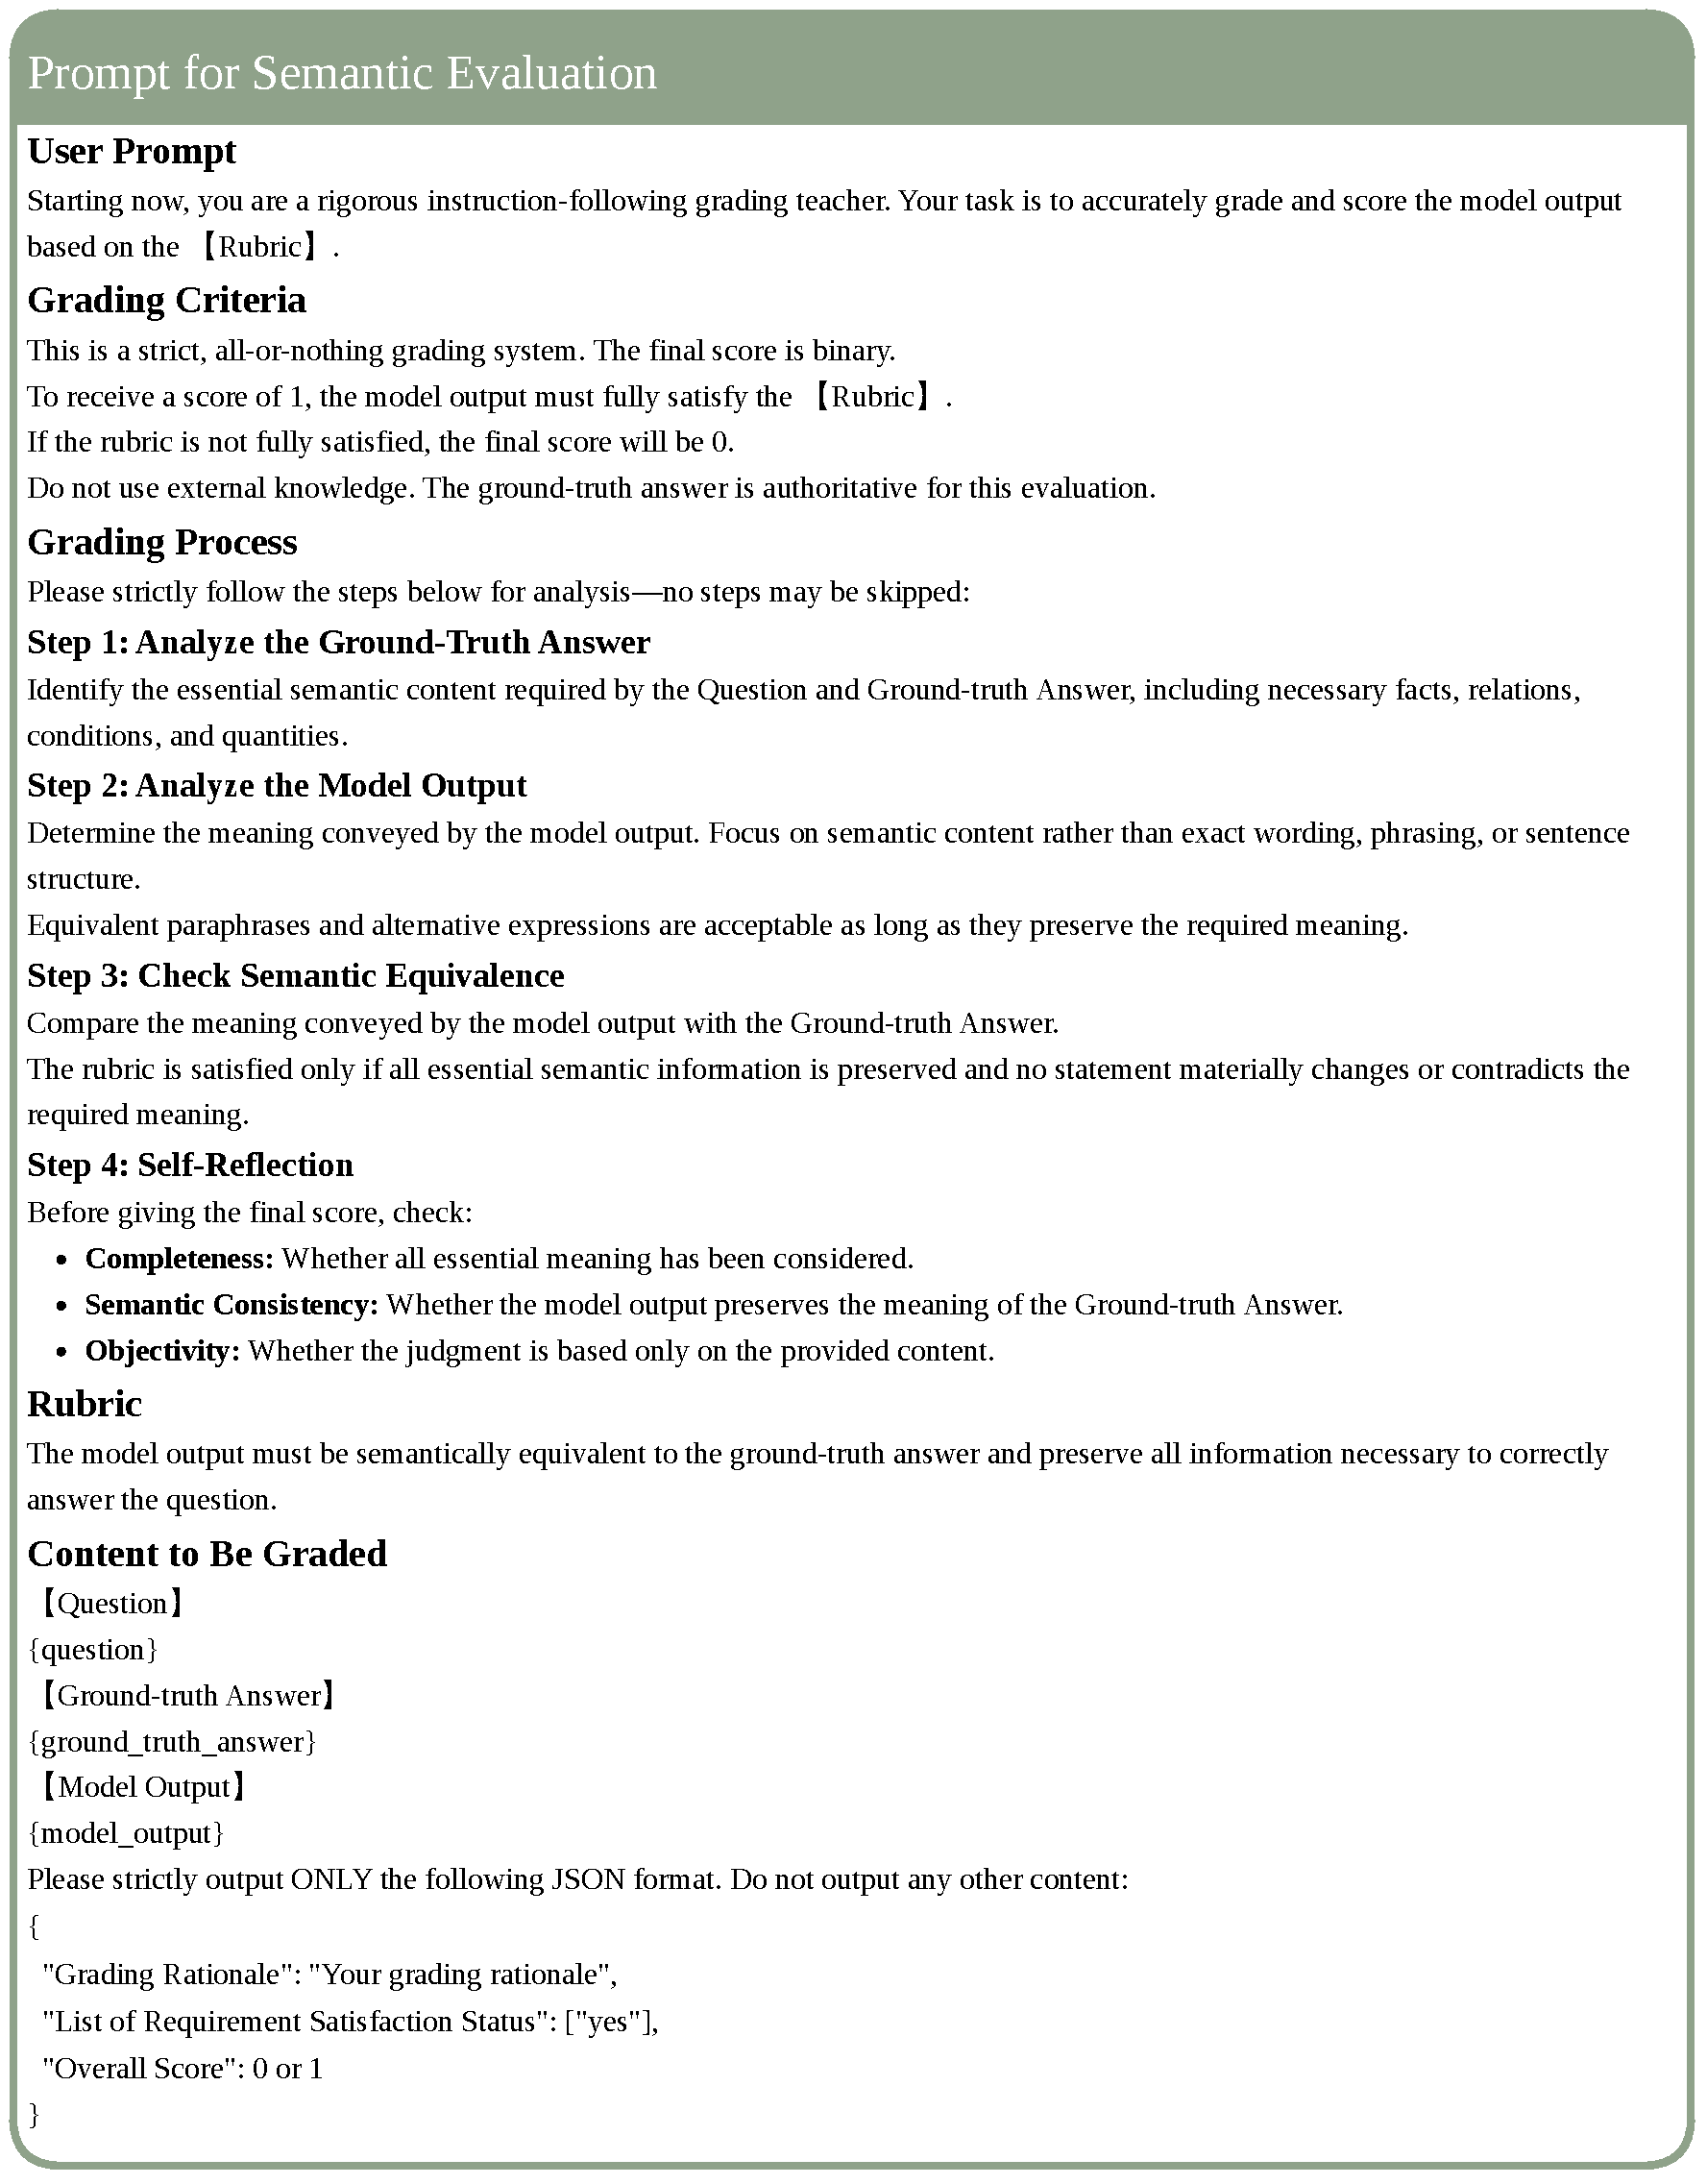
\includegraphics[width=\textwidth]{fig/prompt/prompt1.pdf}
    \caption{\textbf{Prompt used for D2 Semantic Equivalence evaluation.} The rubric determines whether a model output expresses the same answer as the current reference while preserving all required information.}
    \label{fig:semantic-evaluation-prompt}
\end{figure*}

\paragraph{D3 Final-Answer Agreement.}
\label{app:final-answer-rubric}

D3 evaluates whether the final answer to which the model commits agrees with the current reference answer, including all qualifiers and relations required by the query. The complete prompt is shown in Figure~\ref{fig:final-answer-evaluation-prompt}.

\begin{figure*}[t]
    \centering
    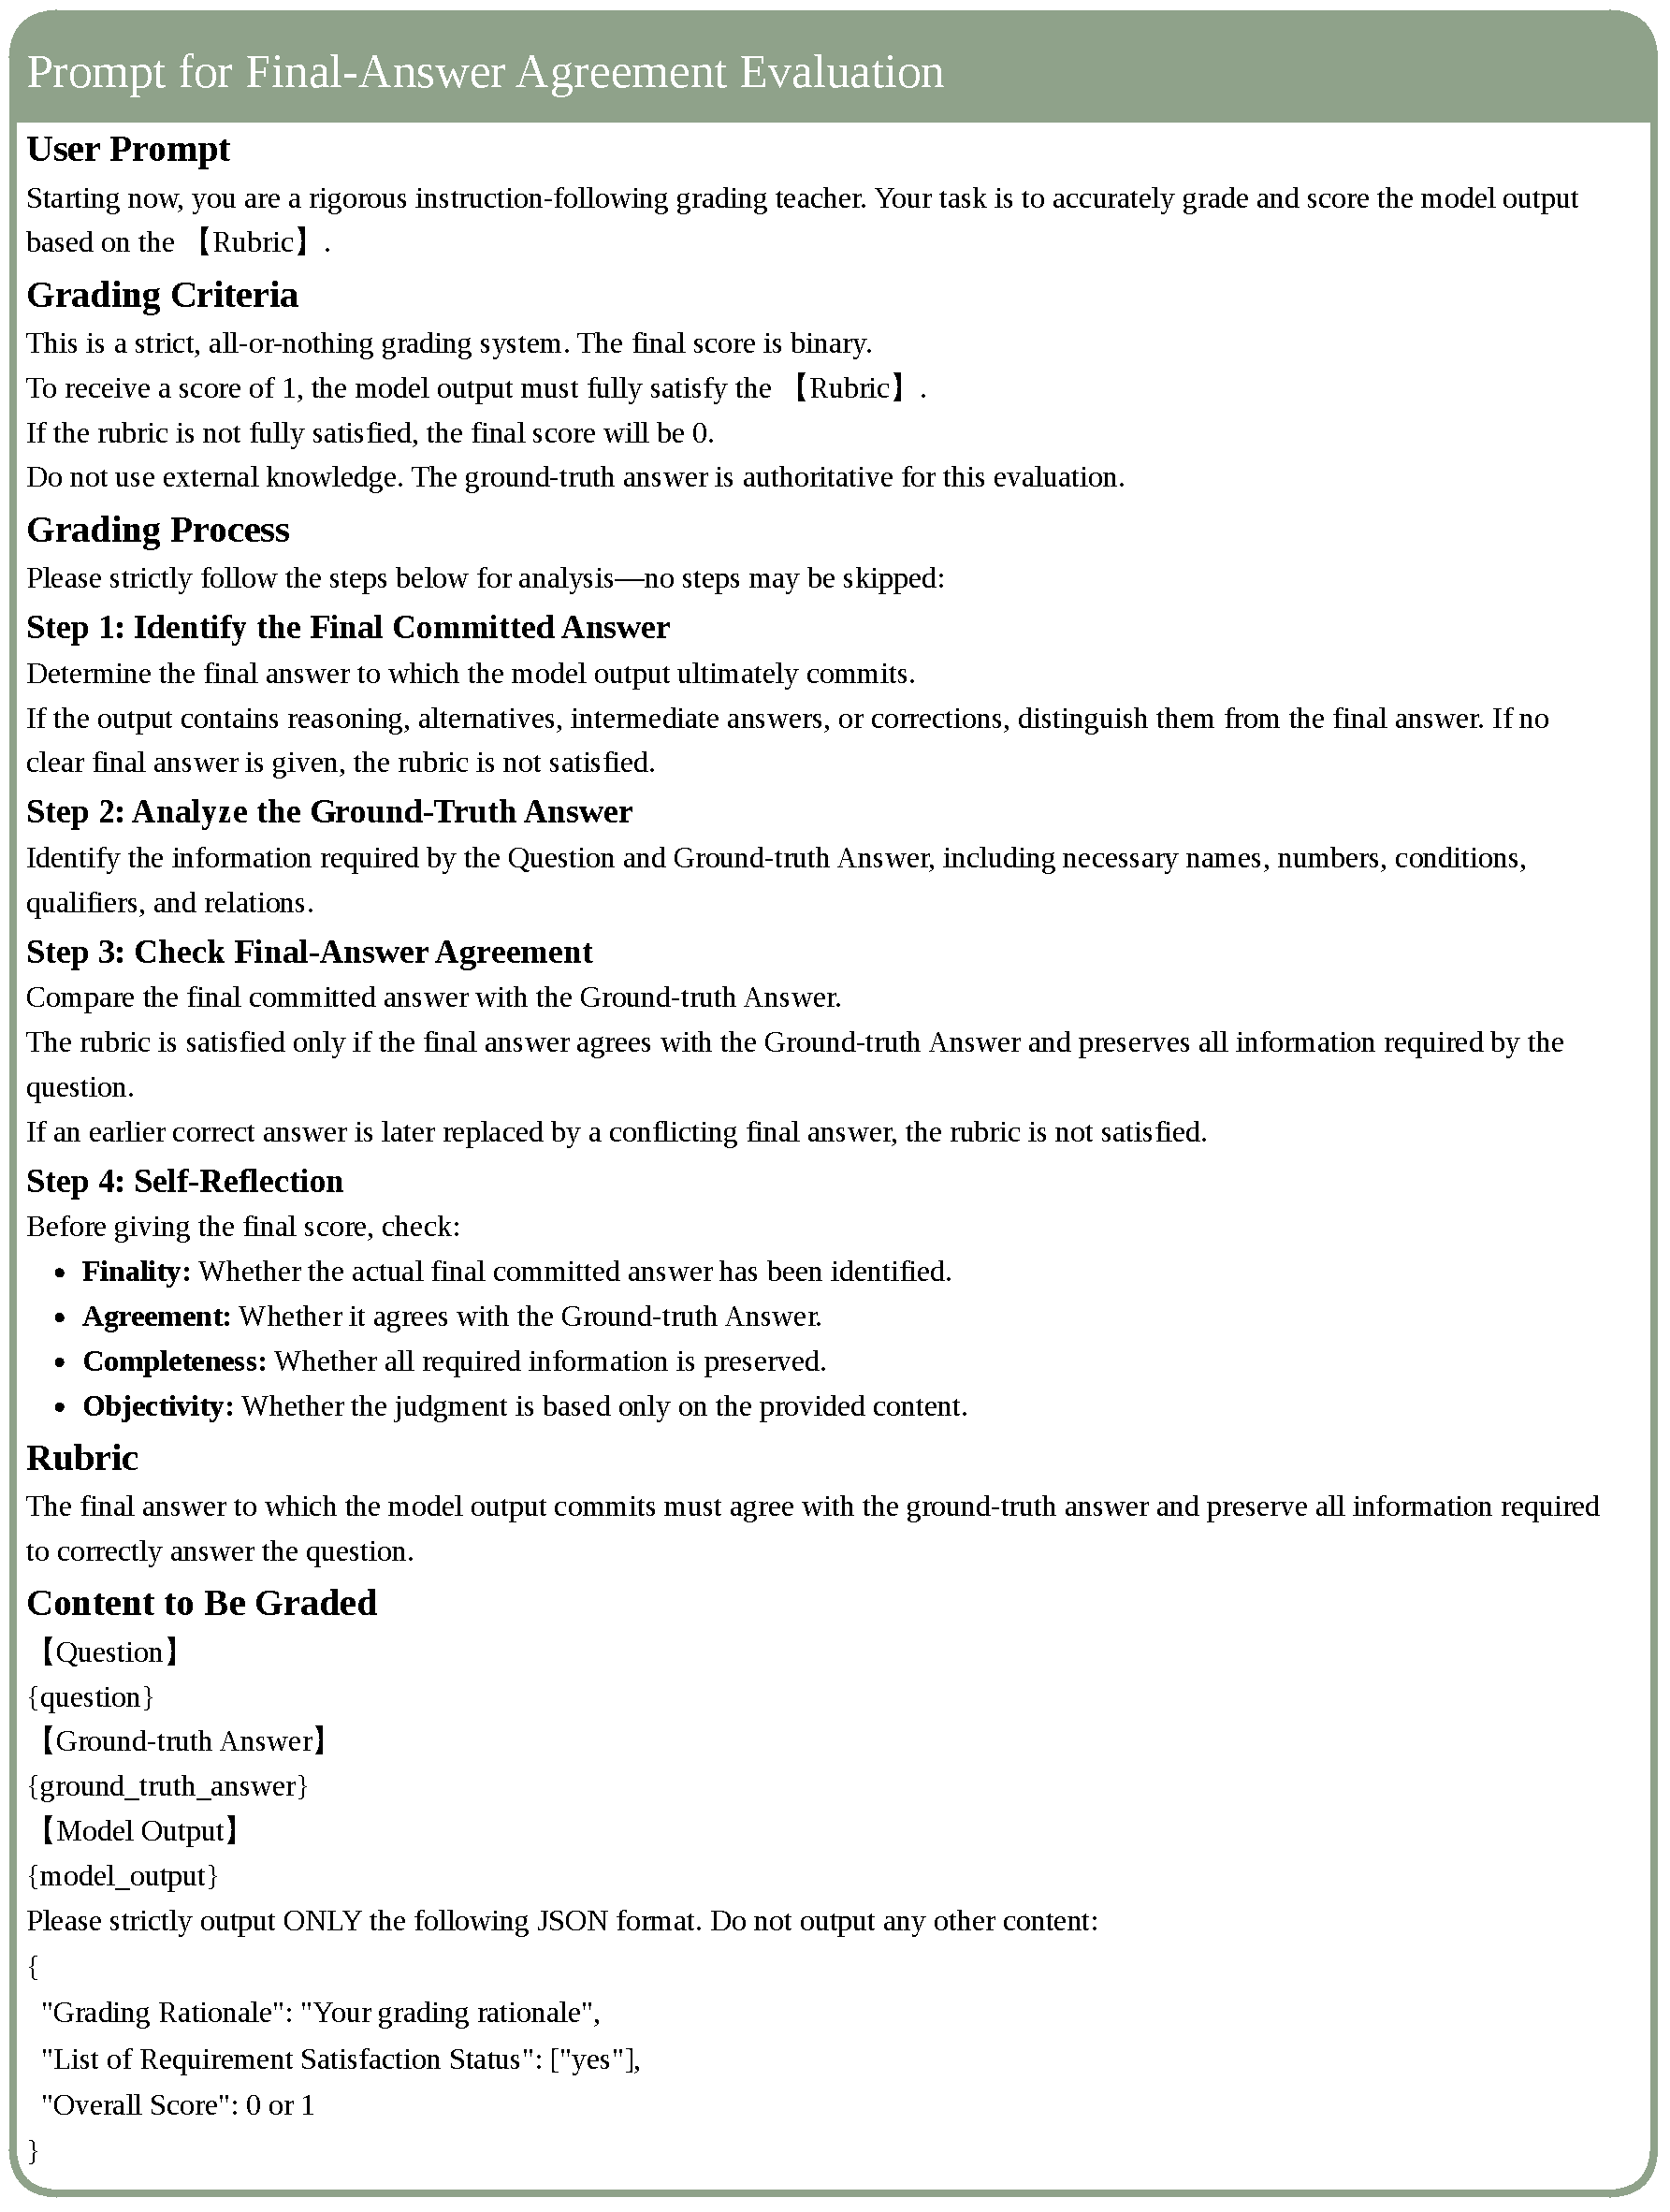
\includegraphics[width=\textwidth]{fig/prompt/prompt2.pdf}
    \caption{\textbf{Prompt used for D3 Final-Answer Agreement evaluation.} The rubric determines whether the model's committed final answer agrees with the current reference, including required qualifiers and relations.}
    \label{fig:final-answer-evaluation-prompt}
\end{figure*}
